\subsection{Far-field scattering} \label{sec:ff_scattering}


\begin{figure}[h] %  figure placement: here, top, bottom, or page
   \centering
   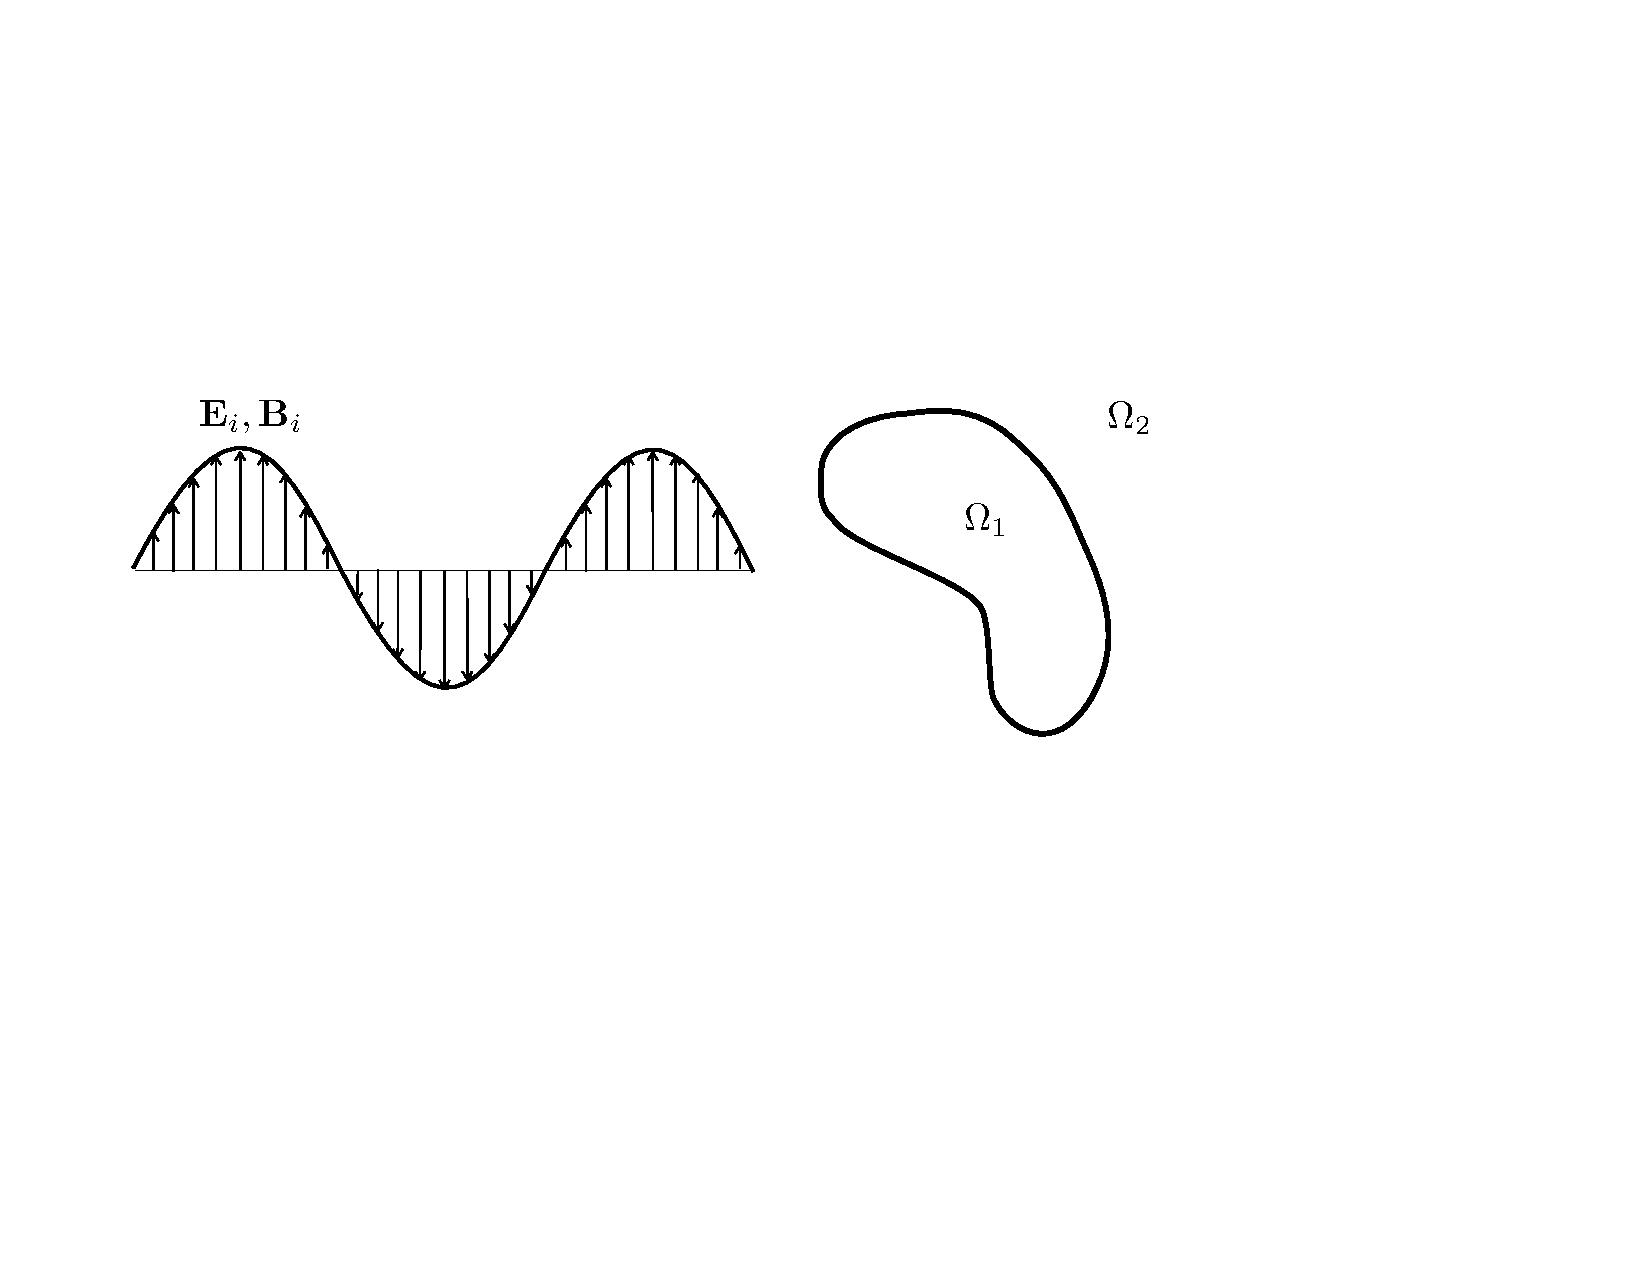
\includegraphics[width=0.49\textwidth]{particle_wave.pdf} 
   \caption{Nanoparticle under electromagnetic wave.}
   \label{fig:part_wave}
\end{figure}

In LSPR computations, we measure the scattered electromagnetic field on a detector
that is located far away from the nanoparticle. When light shines on an object 
like in Figure \ref{fig:part_wave}, the incident wave ($\mathbf{E}_i$,  $\mathbf{B}_i$)
is scattered along the domain, resulting in a total electromagnetic field 
($\mathbf{E}$,  $\mathbf{B}$) that depends on the incoming wave, the particle's 
geometry, and the material constants. In the quasistatic approximation, we only
 need to compute the electric field and the magnetic contribution can be 
neglected \cite{MayergoyzZhang2007}. In the far-field limit, the scattered field
in the outside region ($\Omega_2$) is given by: 

\begin{equation*}
    \mathbf{E}_{2s} = \frac{1}{4\pi\epsilon_2}k^2\frac{e^{ikr}}{r} (\mathbf{\hat{r}} \times \mathbf{p})\times\mathbf{\hat{r}}.
\end{equation*} 

where $k=2\pi/\lambda$ is the wave number and $\lambda$ the wavelength, $\mathbf{\hat{r}}$ 
is a unit vector in the direction of the observation point, and $\mathbf{p}$ is
the dipole moment.

We can also obtain the scattered field with the forward-scattering amplitude \cite{Jackson}:

\begin{equation*}
    \mathbf{E}_{2s}(\mathbf{r})_{r\to\infty} = \frac{e^{ikr}}{r} \mathbf{F}(\mathbf{k},\mathbf{k}_0),
\end{equation*}

where $\mathbf{F}$ is the forward-scattering amplitude, $\mathbf{k}$ is the scattered wave vector in the direction of propagation, and $\mathbf{k}_0$ the wave vector of the incident field. 

Via these two equations, we use \pygbe to compute the scattered electric field 
and then solve for the forward-scattering amplitude. 
